\documentclass{article}
\usepackage[T1]{fontenc}
\usepackage{lmodern}
\usepackage{graphicx}
\usepackage{amsmath,amssymb}
\usepackage[a4paper,margin=2cm]{geometry}
\usepackage[absolute,overlay]{textpos}
\setlength{\TPHorizModule}{1mm}
\setlength{\TPVertModule}{1mm}
\usepackage[indonesian]{babel}
\usepackage{hyperref}
\setlength{\emergencystretch}{2em}
% unit: Halaman 18

\begin{document}

% === Halaman 18 (llm) ===

\section*{World War Steganography}

\begin{itemize}
    \item Penggunaan tinta tak-tampak (\textit{invisible ink}) dalam spionase.
    \begin{itemize}
        \item Pada Perang Dunia II, tinta tak-tampak digunakan untuk menulis pesan rahasia
        \item Tinta terbuat dari campuran susu, sari buah, cuka, dan urine.
        \item Cara membaca: Kertas dipanaskan sehingga tulisan dari tinta tak-tampak tersebut akan menghitam.
    \end{itemize}
\end{itemize}

\vspace{10mm}

Seorang agen FBI sedan menggunakan sinar ultraviolet untuk membaca tulisan yang tersembunyi pada kertas yang dicurigai dari agen spionase.

% deskripsi: Foto hitam putih seorang agen FBI yang sedang menggunakan alat sinar ultraviolet untuk mendeteksi tulisan tersembunyi pada selembar kertas.
% bbox normalisasi: [0.1240, 0.5080, 0.4070, 0.8930]
\begin{textblock*}{59.43mm}(26.04mm,150.88mm)
\noindent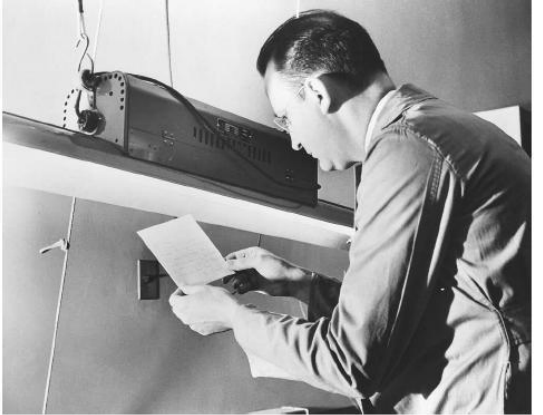
\includegraphics[width=59.43mm,height=114.34mm]{../../images/llm/page_018_img_01.png}%
\end{textblock*}

\end{document}
